\documentclass[../main.tex]{subfiles}
\begin{document}


\section{Experiments and Results} \label{sec:results}

Using the described datasets in section \ref{sec:datasets} the first objective was to determine the general predictive performance of TabNet within the drug discovery domain.

\subsection{Predictive Performance Experiments}

Datasets used were BBBP, BACE, HIV and SIDER, for details refer to section \ref{sec:datasets}. In the following the experiment setup as well as the achieved results are presented. 

\subsubsection{Data Preparation} 

All datasets were randomly split into a training, validation and testing part with a percentage ratio of 80, 10 and 10 within each experiment run. Using the extended-connectivity fingerprint (ECFP) descriptor, molecules in the dataset were represented as a binary matrix in the form of $\mathbf{X} \in \mathbb{B}^{N \times D}$. When using the ECFP molecule descriptor (refer to section \ref{sssec:molecule_descriptors_and_fingerprints}) the folding size defines the number of feature dimension $D$. For $D$ various values were tested. For BBBP $D$ was tested with (512, 4096, 12288), BACE, HIV and SIDER with (512, 4096).

\subsubsection{Baseline} \label{sssec:mlp_baseline}

For direct comparison, a baseline model using a simple MLP utilizing a ReLU activation was trained. Using a Bayesian hyperparameter tuning framework, refer to section \ref{sssec:hyperparameters_search}, the optimal hyperparameter for the baseline MLP were determined first. As a search space dropout probability $p$ was chosen from $[0.0, 0.05, 0.1, 0.3]$, hidden size $H$ chosen between 16 and 256 for 1 up to 8 layers $L$, and the learning rate $\eta$ was defined to be between $0.00001$ and $0.001$. Other fixed hyperparameters were, maximum training steps defined as $1000$, batch size set to 256 and a linear learning rate scheduler with warm up using Adam optimizer was applied. Best hyperparameter were selected out of 25 hyperparameter search runs. All hyperparameters search runs used the same seed for dataset splitting. Early stopping was applied using only the validation dataset part as a guideline. For each of the various feature dimension $D=[512, 4096, 12288]$ hyperparameter search was applied which lead to more than 300 training runs just to deterine the optimal hyperparameter for the corresponding dataset and folding size used. The found hyperparameters for the baseline MLP are presented in the following table \ref{tbl:hyperparameter_mlp}:
\newline

\begin{table}[H]
    \centering
    \begin{tabular}{ |l|l|l|l|l| } 
        \hline
        \rowcolor{lightgray} \textbf{Dataset} & Number Layers & Hidden Size & $\eta$ & Dropout \\
        \hline

        BBBP (D=512)\tablefootnote{Refer to \url{https://mlflow.kriechbaumer.at/#/experiments/73} for all 25 run details} & 4 & 167 & $1.818 \cdot 10^{-5}$ & 0.0 \\
        BBBP (D=4096)\tablefootnote{Refer to \url{https://mlflow.kriechbaumer.at/#/experiments/69} for all 25 run details} & 8 & 44 & $1.724 \cdot 10^{-5}$ & 0.05 \\
        BBBP (D=12288)\tablefootnote{Refer to \url{https://mlflow.kriechbaumer.at/#/experiments/70} for all 25 run details} & 5 & 211 & $1.724 \cdot 10^{-5}$ & 0.1 \\
        
		\hline

		BACE (D=512)\tablefootnote{Refer to \url{https://mlflow.kriechbaumer.at/#/experiments/82} for all 25 run details} & 7 & 150 & $4.722 \cdot 10^{-5}$ & 0.3 \\
		BACE (D=4096)\tablefootnote{Refer to \url{https://mlflow.kriechbaumer.at/#/experiments/87} for all 25 run details} & 1 & 179 & $6.907 \cdot 10^{-5}$ & 0.1 \\

		\hline

		HIV (D=512)\tablefootnote{Refer to \url{https://mlflow.kriechbaumer.at/#/experiments/232} for all 25 run details} & 1 & 232 & $1.97 \cdot 10^{-3}$ & 0.0 \\
		HIV (D=4096)\tablefootnote{Refer to \url{https://mlflow.kriechbaumer.at/#/experiments/235} for all 25 run details} & 1 & 198 & $5.09 \cdot 10^{-5}$ & 0.3 \\

		\hline

		SIDER (D=512)\tablefootnote{Refer to \url{https://mlflow.kriechbaumer.at/#/experiments/253} for all 25 run details} & 2 & 178 & $8.24 \cdot 10^{-3}$ & 0.3 \\
		SIDER (D=4096)\tablefootnote{Refer to \url{https://mlflow.kriechbaumer.at/#/experiments/253} for all 25 run details} & 4 & 189 & $5.16 \cdot 10^{-4}$ & 0.3 \\
    
        \hline
    \end{tabular}
    \caption{Hyperparameter found for MLP baseline models}
 	\label{tbl:hyperparameter_mlp} 	
\end{table}

\subsubsection{TabNet} 

Analog to the baseline model Bayesian hyperparameter search was applied first. Hyperparameter selected were decision size $N_d=[8, 16, 24, 32, 64, 128]$, relaxation parameter $\gamma=[1.0, 1.2, 1.5, 2.0]$, sparsity regularization $\lambda_{sparse}=[0.0, 10^{-6}, 10^{-4}, 0.001, 0.1]$ and the number of decisions steps $N_{steps}$ (between 3 and 10). For the feature transformer the number of shared layers was set to 2 and the number of individual steps to 2. The maximum training steps, batch size, scheduler and optimizer were the same as used within the baseline model. Learning rate was selected within the same range as the baseline model. Batch normalization was not used. Again best hyperparameter were selected out of 25 hyperparameter search runs with the same seed for dataset splitting resulting in over 300 training runs. Early stopping was applied within the hyperparameter search runs. 

\begin{table}[H]
    \centering
    \begin{tabular}{ |l|l|l|l|l|l| } 
        \hline
        \rowcolor{lightgray} \textbf{Dataset} & $N_{steps}$ & $N_d$ & $\gamma$ & $lambda_{sparse}$ & $\eta$ \\
        \hline

        BBBP (D=512)\tablefootnote{Refer to \url{https://mlflow.kriechbaumer.at/#/experiments/54} for all 25 run details} & 5 & 128 & 1.0 & $1.0 \cdot 10^{-6}$ & $3.433 \cdot 10^{-5}$ \\
        BBBP (D=4096)\tablefootnote{Refer to \url{https://mlflow.kriechbaumer.at/#/experiments/61} for all 25 run details} & 8 & 16 & 1.5 & $0.0$ & $6.449 \cdot 10^{-4}$ \\
        BBBP (D=12288)\tablefootnote{Refer to \url{https://mlflow.kriechbaumer.at/#/experiments/59} for all 25 run details} & 6 & 32 & 1.2 & $1.0 \cdot 10^{-3}$ & $8.699 \cdot 10^{-4}$ \\
        
		\hline

		BACE (D=512)\tablefootnote{Refer to \url{https://mlflow.kriechbaumer.at/#/experiments/83} for all 25 run details} & 5 & 24 & 1.5 & 0.0 & $1.0 \cdot 10^{-3}$ \\
        BACE (D=4096)\tablefootnote{Refer to \url{https://mlflow.kriechbaumer.at/#/experiments/86} for all 25 run details} & 4 & 24 & 2.0 & $1.0 \cdot 10^{-6}$ & $3.118 \cdot 10^{-4}$ \\
		
		\hline

		HIV (D=512)\tablefootnote{Refer to \url{https://mlflow.kriechbaumer.at/#/experiments/246} for all 25 run details} & 6 & 128 & 1.5 & 0.0 & $2.48 \cdot 10^{-4}$ \\
        HIV (D=4096)\tablefootnote{Refer to \url{https://mlflow.kriechbaumer.at/#/experiments/261} for all 25 run details} & 3 & 128 & 1.2 & 0.0 & $4.48 \cdot 10^{-4}$ \\
	
		\hline

		SIDER (D=512)\tablefootnote{Refer to \url{https://mlflow.kriechbaumer.at/#/experiments/251} for all 25 run details} & 4 & 64 & 1.5 & $1.0 \cdot 10^{-4}$ & $2.64 \cdot 10^{-3}$ \\
        SIDER (D=4096)\tablefootnote{Refer to \url{https://mlflow.kriechbaumer.at/#/experiments/258} for all 25 run details} & 3 & 24 & 1.0 & $1.0 \cdot 10^{-3}$ & $7.98 \cdot 10^{-4}$ \\
	
        \hline
    \end{tabular}
    \caption{Hyperparameter found for TabNet models}
 	\label{tbl:hyperparameter_tabnet} 	
\end{table}		

\subsubsection{Results} 

The final results have been determined by repeating or retraining each of the experiment setups using selected hyperparameters from scratch 20 times. For each of the experiment runs different random seeds for dataset splitting have been used. The random seed related to the model, e.g. for initialization, stayed the same. The results achieved on the test set can be seen in the following table \ref{tbl:tabnet_bbbp_results} for BBBP, for BACE within table \ref{tbl:tabnet_bace_results} for HIV within table \ref{tbl:tabnet_hiv_results} and for SIDER in table \ref{tbl:tabnet_sider_results}. As metric the mean AUROC and standard deviation of the 20 runs are presented. For additional comparison, results from work by Jiang et al. \cite{jiang_could_2021} as well as a recent result from Ramsauer et al. \cite{ramsauer_hopfield_2020} were used. Both used a similar setup with multiple random split to determine their results.

\begin{table}[H]
    \centering
    \begin{tabular}{ |l|l| } 
        \hline
        \rowcolor{lightgray} \textbf{Model} & \textbf{BBBP mean AUROC ± std} \\
        \hline
        \emph{SVM\cite{jiang_could_2021}} & 0.919 ± 0.028 \\
		\emph{XGBoost\cite{jiang_could_2021}} & 0.926 ± 0.026 \\
		\emph{RF\cite{jiang_could_2021}} & \textbf{0.927 ± 0.025} \\
		\emph{GCN\cite{jiang_could_2021}} & 0.903 ± 0.027 \\
		\emph{GAT\cite{jiang_could_2021}} & 0.898 ± 0.033 \\
		\emph{DNN\cite{jiang_could_2021}} & 0.898 ± 0.033 \\
		\emph{MPNN\cite{jiang_could_2021}} & 0.879 ± 0.030 \\
		\emph{Attentive FP\cite{jiang_could_2021}} & 0.887 ± 0.032 \\
		\emph{Hopfield\cite{ramsauer_hopfield_2020}} & 0.910 ± 0.026 \\

        \hline
        \textbf{TabNet} ($D=512$)\tablefootnote{Refer to \url{https://mlflow.kriechbaumer.at/#/experiments/56} for all 20 run details} & 0.874 ± 0.032 \\
        \textbf{TabNet} ($D=4096$)\tablefootnote{Refer to \url{https://mlflow.kriechbaumer.at/#/experiments/63} for all 20 run details} & 0.875 ± 0.022 \\
        \textbf{TabNet} ($D=12288$)\tablefootnote{Refer to \url{https://mlflow.kriechbaumer.at/#/experiments/62} for all 20 run details} & 0.891 ± 0.030 \\

        \hline
        \textbf{Baseline MLP} ($D=512$)\tablefootnote{Refer to \url{https://mlflow.kriechbaumer.at/#/experiments/74} for all 20 run details} & 0.877 ± 0.032 \\
        \textbf{Baseline MLP} ($D=4096$)\tablefootnote{Refer to \url{https://mlflow.kriechbaumer.at/#/experiments/71} for all 20 run details} & 0.902 ± 0.022 \\
        \textbf{Baseline MLP} ($D=12288$)\tablefootnote{Refer to \url{https://mlflow.kriechbaumer.at/#/experiments/72} for all 20 run details} & 0.913 ± 0.022 \\
        
     \hline
    \end{tabular}
    \caption{TabNet results on BBBP test set showing mean AUROC ± standard deviation for 20 random splits}
 	\label{tbl:tabnet_bbbp_results} 	
\end{table}

\begin{table}[H]
    \centering
    \begin{tabular}{ |l|l| } 
        \hline
        \rowcolor{lightgray} \textbf{Model} & \textbf{BACE mean AUROC ± std} \\
        \hline

        \emph{SVM\cite{jiang_could_2021}} & 0.893 ± 0.020 \\
		\emph{XGBoost\cite{jiang_could_2021}} & 0.889 ± 0.021 \\
		\emph{RF\cite{jiang_could_2021}} & 0.890 ± 0.022 \\
		\emph{GCN\cite{jiang_could_2021}} & 0.898 ± 0.019 \\
		\emph{GAT\cite{jiang_could_2021}} & 0.886 ± 0.023 \\
		\emph{DNN\cite{jiang_could_2021}} & 0.890 ± 0.024 \\
		\emph{MPNN\cite{jiang_could_2021}} & 0.838 ± 0.027 \\
		\emph{Attentive FP\cite{jiang_could_2021}} & 0.876 ± 0.023 \\
		\emph{Hopfield\cite{ramsauer_hopfield_2020}} & \textbf{0.902 ± 0.023} \\

        \hline
        \textbf{TabNet} ($D=512$)\tablefootnote{Refer to \url{https://mlflow.kriechbaumer.at/#/experiments/85} for all 20 run details} & 0.858 ± 0.029 \\
        \textbf{TabNet} ($D=4096$)\tablefootnote{Refer to \url{https://mlflow.kriechbaumer.at/#/experiments/89} for all 20 run details} & 0.854 ± 0.032 \\    
        \hline   
        \textbf{Baseline MLP} ($D=512$)\tablefootnote{Refer to \url{https://mlflow.kriechbaumer.at/#/experiments/84} for all 20 run details} & 0.876 ± 0.033 \\
        \textbf{Baseline MLP} ($D=4096$)\tablefootnote{Refer to \url{https://mlflow.kriechbaumer.at/#/experiments/88} for all 20 run details} & 0.893 ± 0.032 \\
    
        \hline
    \end{tabular}
    \caption{TabNet results on BACE test set showing mean AUROC ± standard deviation for 20 random splits}
 	\label{tbl:tabnet_bace_results} 	
\end{table}

\begin{table}[H]
    \centering
    \begin{tabular}{ |l|l| } 
        \hline
        \rowcolor{lightgray} \textbf{Model} & \textbf{HIV mean AUROC ± std} \\
        \hline

        \emph{SVM\cite{jiang_could_2021}} & 0.822 ± 0.020 \\
		\emph{XGBoost\cite{jiang_could_2021}} & 0.816 ± 0.020 \\
		\emph{RF\cite{jiang_could_2021}} & 0.820 ± 0.016 \\
		\emph{GCN\cite{jiang_could_2021}} & \textbf{0.834 ± 0.025} \\
		\emph{GAT\cite{jiang_could_2021}} & 0.826 ± 0.030 \\
		\emph{DNN\cite{jiang_could_2021}} & 0.797 ± 0.018 \\
		\emph{MPNN\cite{jiang_could_2021}} & 0.811 ± 0.031 \\
		\emph{Attentive FP\cite{jiang_could_2021}} & 0.822 ± 0.026 \\
		\emph{Hopfield\cite{ramsauer_hopfield_2020}} & 0.815 ± 0.023 \\

        \hline
        \textbf{TabNet} ($D=512$)\tablefootnote{Refer to \url{https://mlflow.kriechbaumer.at/#/experiments/248} for all 20 run details} & 0.752 ± 0.028 \\
        \textbf{TabNet} ($D=4096$)\tablefootnote{Refer to \url{https://mlflow.kriechbaumer.at/#/experiments/262} for all 20 run details} & 0.755 ± 0.019  \\    
        \hline   
        \textbf{Baseline MLP} ($D=512$)\tablefootnote{Refer to \url{https://mlflow.kriechbaumer.at/#/experiments/238} for all 20 run details} & 0.775 ± 0.027 \\
        \textbf{Baseline MLP} ($D=4096$)\tablefootnote{Refer to \url{https://mlflow.kriechbaumer.at/#/experiments/237} for all 20 run details} & 0.785 ± 0.024 \\
    
        \hline
    \end{tabular}
    \caption{TabNet results on HIV test set showing mean AUROC ± standard deviation for 20 random splits}
 	\label{tbl:tabnet_hiv_results} 	
\end{table}

\begin{table}[H]
    \centering
    \begin{tabular}{ |l|l| } 
        \hline
        \rowcolor{lightgray} \textbf{Model} & \textbf{SIDER mean AUROC ± std} \\
        \hline

        \emph{SVM\cite{jiang_could_2021}} & 0.630 ± 0.021 \\
		\emph{XGBoost\cite{jiang_could_2021}} & 0.642 ± 0.020 \\
		\emph{RF\cite{jiang_could_2021}} & 0.646 ± 0.022 \\
		\emph{GCN\cite{jiang_could_2021}} & 0.634 ± 0.026 \\
		\emph{GAT\cite{jiang_could_2021}} & 0.627 ± 0.024 \\
		\emph{DNN\cite{jiang_could_2021}} & 0.631 ± 0.028 \\
		\emph{MPNN\cite{jiang_could_2021}} & 0.598 ± 0.031 \\
		\emph{Attentive FP\cite{jiang_could_2021}} & 0.623 ± 0.026 \\
		\emph{Hopfield\cite{ramsauer_hopfield_2020}} & \textbf{0.672 ± 0.019} \\

        \hline
        \textbf{TabNet} ($D=512$)\tablefootnote{Refer to \url{https://mlflow.kriechbaumer.at/#/experiments/252} for all 20 run details} & 0.588 ± 0.032 \\
        \textbf{TabNet} ($D=4096$)\tablefootnote{Refer to \url{https://mlflow.kriechbaumer.at/#/experiments/259} for all 20 run details} & 0.582 ± 0.027 \\    
        \hline   
        \textbf{Baseline MLP} ($D=512$)\tablefootnote{Refer to \url{https://mlflow.kriechbaumer.at/#/experiments/254} for all 20 run details} & 0.629 ± 0.028 \\
        \textbf{Baseline MLP} ($D=4096$)\tablefootnote{Refer to \url{https://mlflow.kriechbaumer.at/#/experiments/257} for all 20 run details} & 0.644 ± 0.018 \\
    
        \hline
    \end{tabular}
    \caption{TabNet results on SIDER test set showing mean AUROC ± standard deviation for 20 random splits}
 	\label{tbl:tabnet_sider_results} 	
\end{table}

\subsection{Interpretability Experiment} \label{ssec:interpret_experiment}

The second part of the experiments uses the hERG dataset and identified relevant components, refer to section \ref{ssec:herg_dataset}, in an attempt to empirically analyze TabNets interpretability capabilities, using the feature selection mask, to identify and rank most relevant features. The experiment setup follows the approach from Schimunek J. et al. \cite{schimunek_poster_2021} and uses hERG identified relevant components as a ground truth for most relevant features. The experiment setup is explained in the following sections.

\subsubsection{Data Preparation} 

hERG dataset was split in a ratio of 60:20:20 for training, validation and testing parts. Molecules were represented in a combination of extended-connectivity fingerprints (ECFP) with a folding size of $D_{ecfp}=1024$, MACCS fingerprints $D_{m}=167$ and 826 SMARTS (refer to section \ref{sssec:molecule_descriptors_and_fingerprints}) pattern from Mayr A. et al. \cite{DeepTox} with $D_{t}=826$. This resulted in a combined feature dimension of $D=2017$ and input data $\mathbf{X} \in \mathbb{R}^{B \times 2017}$ with $B$ as the batch size.

\subsubsection{Atomic Attribution and Mapping}

Each molecule $mol_{i}$ consists of $J_i$ individual atoms which vary from molecule to molecule. Using a descriptor one molecule $i$ can be represented as a vector $\mathbf{x_i} \in \mathbb{R}^{D}$. $D$ depends on the descriptor and corresponding settings used. The descriptor is a function mapping from molecule and its atomic structure to its numerical representation in the form of $d \mid mol_i \rightarrow \mathbb{R}^D$. In similar way a atomic contribution mapping can be identified using a mapping function $m \mid \mathbb{R}^D \rightarrow \mathbb{R}^{J_i}$ for each descriptor. This mapping describes each feature dimension $d$ and its contribution factor to each atom $j$.
Using a feature attribution methods for a trained model, for example as given by TabNets feature masks $\mathbf{M_{agg}}$ (section \ref{sssec:interpretability}) or other feature attributions methods (section \ref{ssec:interpret_methods}) the feature attribution $\mathbf{v_i} \in \mathbb{R}^{D}$ for one particular molecule $i$ can be identified. Using the atomic mapping function $m(\mathbf{v_i})$ one can calculate the atomic attribution $\mathbf{a_i} \in \mathbb{R}^{J_i}$ for a particular molecule $i$ for each descriptor. When using multiple molecule descriptors (as in this experiment setup) the overall atomic attribution for one particular molecule $i$ is given by the sum of all atomic attribution over all descriptors. 

In the following figure \ref{fig:atomic_mapping_sample} the atomic mapping for one concrete sample of the hERG dataset with 20 heavy atoms (D2392 with smile "O1c2c(C(=O)C[C@H]1c1ccc(O)cc1) c(O)cc(O)c2" and IUPAC name "(2S)-5,7-dihydroxy-2-( 4-hydroxyphenyl)chroman-4-one") which is hERG inactive is shown. In the example an ECFP fingerprint is used with an unrealistic folding size of 32 and radius of 1 for visualization purpose. The strength of each individual edge indicates the different factors for individual contribution of one feature dimension to the actual atom. Furthermore in figure \ref{fig:atomic_attribution_sample} the same atom with a given atomic attribution is presented using feature attributions (e.g. from TabNet or other feature attribution methods). Using the mapping function $m$ presented in the form of edges the concrete atomic attribution for each atom within the hERG inactive sample is determined.

\begin{figure}[H]
    \centering
    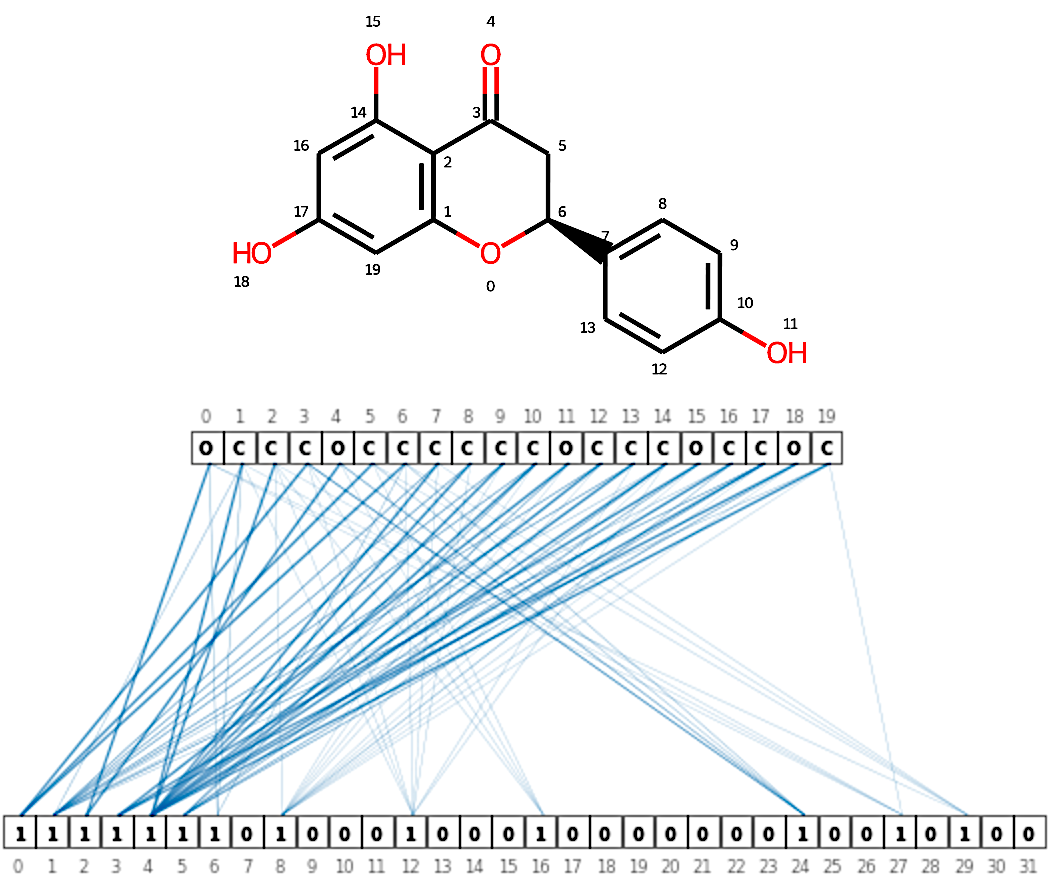
\includegraphics[width=0.8\textwidth]{atomic_mapping_sample}    
    \caption{Atomic mapping example showing one hERG inactive molecule sample. On top a hERG inactive molecule including atom indices is presented. The bottom gives a sample for the corresponding ECFP fingerprint.}
    \label{fig:atomic_mapping_sample}
\end{figure}

\begin{figure}[H]
    \centering
    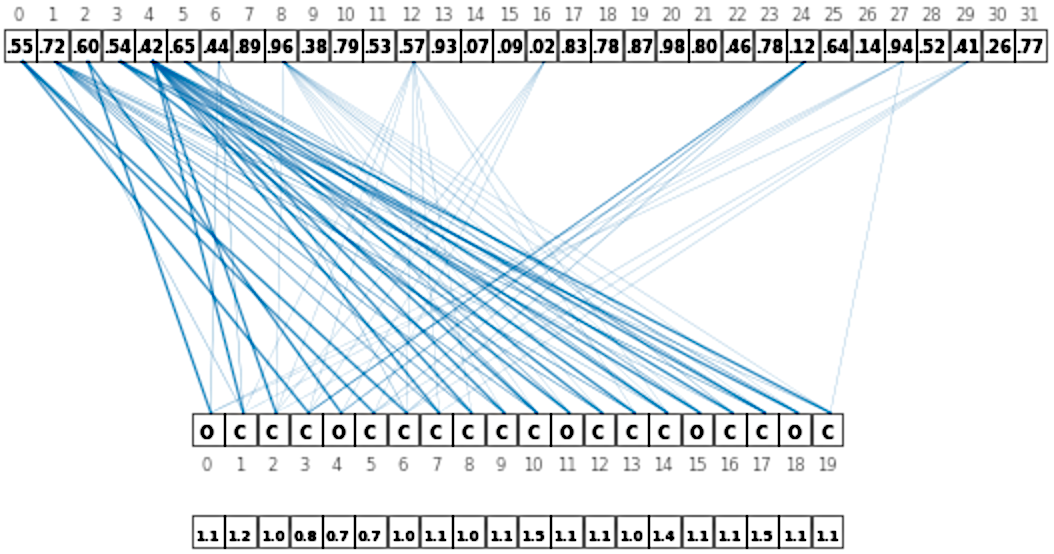
\includegraphics[width=0.8\textwidth]{atomic_attribution_sample}    
    \caption{Atomic attribution example for one hERG inactive molecule sample. On top the feature attribution is given and on bottom the calculated atomic attribution}
    \label{fig:atomic_attribution_sample}
\end{figure}

The implementation of the individual mapping functions $m$ for each descriptor type (ECFP, MACCSkeys, and DeepTox \cite{DeepTox}) was kindly provided by Schimunek J. \cite{schimunek_poster_2021}. As the determination of the atomic mapping is computational expensive, due to the fact that the atomic mapping is individual per molecule and descriptor, within this master thesis work the atomic mapping was precomputed and cached. The atomic mapping stores the information which feature dimension of a descriptor contributes to which atom index by what factor. The blue edges in figure \ref{fig:atomic_mapping_sample} refer a sample atomic mapping which can be precomputed and cached. Given feature attributions using the precomputed atomic mapping the atomic attribution can be calculated without the usage of the actual mapping function $m$. This significantly improves experiment runtime. 

\subsubsection{Metric and Evaluation Methodology} \label{sssec:evaluation_methodology}

To evaluate the identified atomic attribution the hERG identified relevant substructures, as described in section \ref{ssec:herg_dataset}, are used as a ground truth. A perfect atomic attribution would attribute and rank those atom indices higher which do match a relevant ground truth substructure. To measure the ability to rank atomic attribution which match a relevant substructure the area under the receiver operator characteristic curve (AUROC) was used. To illustrate this, in figure \ref{fig:atomic_relevant_attribution_sample} the hERG relevant substructure Ethoxybenzene (with smile "CCOc1ccccc1") is presented matching a hERG molecule (same as given in figure \ref{fig:atomic_mapping_sample}) at atom indices indicated in red. 

\begin{figure}[H]
    \centering
    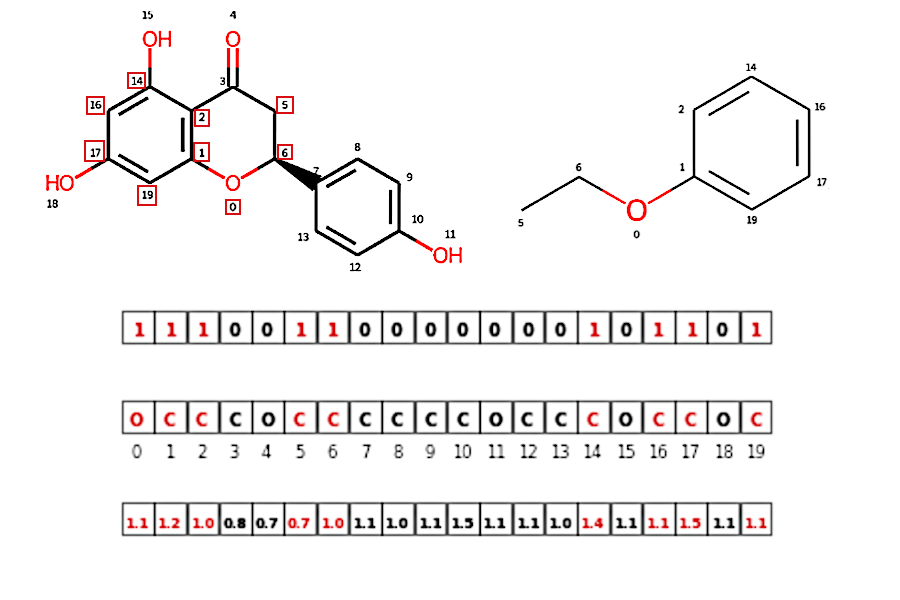
\includegraphics[width=0.8\textwidth]{atomic_relevant_attribution_sample}    
    \caption{hERG relevant substructure matching. Top left shows a large hERG molecule with a matching relevant substructure to its right. Matching atomic indices are marked in red. On bottom the relevant numerical atomic attribution is given.}
    \label{fig:atomic_relevant_attribution_sample}
\end{figure} 

Using the determined atomic attribution the AUROC between the matching atom indices represented by the binary vector $\mathbf{s}$ and atomic attribution $\mathbf{a}$

\begin{equation}
\nonumber
\begin{split}
    \mathbf{s} & = [\color{red}1.0, \color{red}1.0, \color{red}1.0, \color{gray}0.0, \color{gray}0.0, \color{red}1.0, \color{red}1.0, \color{gray}0.0, \color{gray}0.0, \color{gray}0.0, \color{gray}0.0, \color{gray}0.0, \color{gray}0.0, \color{gray}0.0, \color{red}1.0, \color{gray}0.0, \color{red}1.0, \color{red}1.0, \color{gray}0.0, \color{red}1.0\color{gray}] \\
    \mathbf{a} & = [\color{red}1.1, \color{red}1.2, \color{red}1.0, \color{gray}0.8, \color{gray}0.7, \color{red}0.7, \color{red}1.0, \color{gray}1.1, \color{gray}1.0, \color{gray}1.1, \color{gray}1.5, \color{gray}1.1, \color{gray}1.1, \color{gray}1.0, \color{red}1.4, \color{gray}1.1, \color{red}1.1, \color{red}1.5, \color{gray}1.1, \color{red}1.1\color{gray}]
\end{split}
\end{equation}

is $0.59$. 
As reference for intuition, a perfect atomic attribution ranking on a fictive sample having $\mathbf{s} = [0, 1, 0, 0, 1]$ could be $\mathbf{a} = $[0.5, 0.7, 0.3, 0.1, 0.6] with AUROC of $1.0$ while a worst case scenario could be given $\mathbf{a} = [0.5, 0.7, 0.3, 0.0, 0.6]$ with AUROC of $0.0$.
\newline

% Using the determined atomic attribution the AUROC between the matching atom indices represented by the binary vector $\mathbf{s} = $[1, 1, 1, 0, 0, 1, 1, 0, 0, 0, 0, 0, 0, 0, 1, 0, 1, 1, 0, 1] and the atomic attribution $\mathbf{a} = $[1.1, 1.2, 1.0, 0.8, 0.7, 0.7, 1.0, 1.1, 1.0, 1.1, 1.5, 1.1, 1.1, 1.0, 1.4, 1.1, 1.1, 1.5, 1.1, 1.1] in figure \ref{fig:atomic_relevant_attribution_sample} is $0.59$. As reference for intuition, a perfect atomic attribution ranking on a fictive sample having $\mathbf{s} = [0, 1, 0, 0, 1]$ could be $\mathbf{a} = $[0.5, 0.7, 0.3, 0.1, 0.6] with AUROC of $1.0$ while a worst case scenario could be given $\mathbf{a} = [0.5, 0.7, 0.3, 0.0, 0.6]$ with AUROC of $0.0$.

Given the described methodology using the AUROC to determine the ability to rank relevant atoms based on their atomic attribution first, as ground truth only unique hERG active substructures were considered. Those hERG active substructures (also refer to table \ref{tbl:hergophores}) are ethoxybenzene (smile "CCOc1ccccc1"), N-methyl-2-phenylethanamine (smile "c1ccccc1CCNC"), 1-(phenylmethyl)piperidine (smile "c1ccccc1CN2CCCCC2"), N-(phenylmethyl)ethanamine (smile "c1ccccc1CNCC") and phenylmethylbenzene (smile "c1ccccc1Cc1ccccc1"). Using those 5 ground truth molecules the final score was calculated as follows:

\begin{enumerate}
	\item Train model using the hERG dataset with the binary classification objective of a molecule being either hERG active or inactive (only the first target of the hERG dataset as described in section \ref{ssec:herg_dataset} was considered).
	\item Get all hERG activity predictions for the test part of the dataset using the trained model.
	\item Calculate the feature attributions using a feature attribution method (e.g. TabNet $M_{agg}$ or methods described in section \ref{ssec:interpret_methods})
	\item Use the feature attributions to get all atomic attributions utilizing the precomputed and cached atomic mappings.
	\item Consider samples for which the hERG activity was predicted as inactive. 
	\item For all those samples calculate the ranking score (AUROC) using the atomic attributions on each ground truth molecule (5 relevant substructures). Obviously the value is only calculated if the ground truth molecule is indeed a substructure of a particular hERG molecule.
	\item The final score is the mean over all the individual ranking scores for each hERG sample and potential substructure. 
\end{enumerate}

This process, using the inactive hERG predictions together with substructures which are most relevant for hERG active molecules, might seam to be non-intuitive but follows the counterfactual thinking approach anaolog to the setup used by Schimunek et al. \cite{schimunek_poster_2021}. The idea is that despite of one molecule being predicted as hERG inactive the typically substructure found in hERG active molecules should still be considered important. 

\subsubsection{Training}

The experiment setup and evaluation methodology was applied onto different ML model architectures and feature interpretability methods. This allows for a broader picture and gives reference results for TabNets interpretability capabilities. Additionally this follows the work of Schimunek et al. \cite{schimunek_poster_2021} in which interpretability methods were first empirically evaluated using the hERG dataset with a trained MLP as a bases.
For model architectures \textbf{TabNet}, using the reimplementation described in section \ref{sssec:tabnet_implementation_details}, a \textbf{Baseline MLP}, using the same baseline implementation as described in section \ref{sssec:mlp_baseline}, \textbf{Random Forest (RF)}\footnote{Using the scikit-learn implementation \cite{scikit-learn}} and \textbf{Gradient Boosting Decision Tree (GBDT)}\footnote{Using the XGBoost implementation \cite{chen_xgboost_2016}} were evaluated.

Given the model architectures the following combinations of interpretability methods were evaluated.

\begin{itemize}
	\item \textbf{TabNets $M_{agg}$} - only used and relevant for the TabNet architecture
	\item \textbf{Integrated Gradients (IG)}\footnote{Using the captum implementation \cite{kokhlikyan2020captum}} - applied after training \emph{TabNet} and a baseline \emph{MLP}
	\item \textbf{Saliency (absolute and relative)}\footnotemark[\value{footnote}] - applied after training \emph{TabNet} and a baseline \emph{MLP}
	\item \textbf{Input $\times$ Gradient}\footnotemark[\value{footnote}] - applied after training \emph{TabNet} and a baseline \emph{MLP}
	\item \textbf{Shapley Value Sampling}\footnotemark[\value{footnote}] - applied for all model types
	
	%\footnotetext

	%\item \emph{Tree Interpreter}\footnote{Using the implemenation by Saabas Ando \cite{saabas_treeinterpreter_2021}} - applied to RF
\end{itemize}

Before any interpretability method was applied to evaluate interpretability capabilities as described in section \ref{sssec:evaluation_methodology} for each model type hyperparameter search using Bayesian hyperparameter optimization as described in section \ref{sssec:hyperparameters_search} was applied. For each model architecture the following optimal hyperparameters were determined over 30 trials each.

\begin{itemize}

	\item \textbf{TabNet} - The best found TabNet architecture\footnote{Refer to \url{https://mlflow.kriechbaumer.at/#/experiments/212} for all 30 trials} uses 3 decision steps with decision size $N_d=16$, $\gamma=1.5$ and $\lambda_{sparse}=10^{-4}$ for sparsity regularization. As learning rate $0.01$ was determined with a batch size of 256. AdamW optimizer with weight decay of $0.0001$ together with an exponential decaying learning rate scheduler having decaying rate $\beta=0.9$ over 800 steps was applied. Batch normalization was applied using momentum $0.95$ and a virtual batch size for ghost batch norm of $64$. 

	\item \textbf{Baseline MLP} - The best found architecture\footnote{Refer to \url{https://mlflow.kriechbaumer.at/#/experiments/205} for all 30 trials} is a 3 layer MLP with hidden size of $128$. Dropout was not applied. Batch normalization was determined with a momentum of $0.9$. Model was trained with a batch size of $512$ using Adam without weight decay utilizing a linear scheduler with a maximum learning rate of $0.001$.

	\item \textbf{Random Forest (RF)} - The best RF found\footnote{Refer to \url{https://mlflow.kriechbaumer.at/#/experiments/217} for all 30 trials} consists of 200 decision trees. Bootstrap sampling was not applied. The splitting criteria used was entropy or information gain as described in section \ref{ssec:dt}. The minimum amount of samples for one split was determined to be 5 with at least 2 samples per split leaf. For the maximum number of features considered, the square root of feature dimensions (in this case $\sqrt{2017}$) or around $44$ for the hERG dataset was determined. The maximum depth of one decision tree was set to 40.

	\item \textbf{Gradient Boosting Decision Tree (GBDT)} - The best GBDT found\footnote{Refer to \url{https://mlflow.kriechbaumer.at/#/experiments/220} for all 30 trials} uses learning rate of $0.1$ for boosting and has a maximum depth of 24 per decision tree trained. 

\end{itemize}

\subsubsection{Results}

Given the optimal hyperparameters found each model architecture was repeatedly trained using 20 different random splits of the hERG dataset. In the following table \ref{tbl:herg_results} the result of the binary classification task whether a molecule is hERG active or inactive is presented using the mean AUROC as well as the standard deviation on the test part over 20 consecutive random splits.

\begin{table}[H]
    \centering
    \begin{tabular}{ |l|l|l|l| } 
        \hline
        \rowcolor{lightgray} \textbf{Model} & \textbf{hERG mean AUROC ± std} & min AUROC & max AUROC \\
        \hline       

        \hline
        \textbf{TabNet}\tablefootnote{Refer to \url{https://mlflow.kriechbaumer.at/#/experiments/214} for all 20 run details} & 0.826 ± 0.017 & 0.793 & 0.859 \\
        
        \textbf{MLP}\tablefootnote{Refer to \url{https://mlflow.kriechbaumer.at/#/experiments/211} for all 20 run details} & 0.878 ± 0.010 & 0.864 & 0.895 \\    
        
        \textbf{RF} & \textbf{0.895 ± 0.008} & 0.879 & 0.916 \\
        
        \textbf{GBDT}\tablefootnote{Refer to \url{https://mlflow.kriechbaumer.at/#/experiments/222} for all 20 run details} & 0.890 ± 0.009 & 0.877 & 0.903 \\
    
        \hline
    \end{tabular}
    \caption{Comparative results on hERG test set showing mean AUROC ± standard deviation for 20 random splits}
 	\label{tbl:herg_results} 	
\end{table}

After each consecutive training runs the mentioned interpretability methods were applied using the trained models using the methodology described in section \ref{sssec:evaluation_methodology}. In the following tables \ref{tbl:herg_tabnet_interpret_results}, \ref{tbl:herg_mlp_interpret_results} and \ref{tbl:herg_dt_interpret_results} the achieved score (using AUROC) ranking relevant atoms first is presented. Methods are ordered descending from best to worst achieved performance. TabNets performance is shown in table \ref{tbl:herg_tabnet_interpret_results}.

\begin{table}[H]
    \centering
    \begin{tabular}{ |l|l|l|l| } 
        \hline
        \rowcolor{lightgray} \textbf{Interpretability Method}\tablefootnote{Refer to \url{https://mlflow.kriechbaumer.at/#/experiments/214} for all 20 run details} & \textbf{mean AUROC ± std} & min AUROC & max AUROC \\
        \hline       

        \hline
        Shapley Value Sampling & \textbf{0.649 ± 0.069} & 0.451 & 0.727 \\
        
        Integrated Gradients (IG) & 0.637 ± 0.069 & 0.465 & 0.721 \\    
        
        Input $\times$ Gradient & 0.611 ± 0.041 & 0.523 & 0.683 \\

        Saliency (relative) & 0.534 ± 0.023 & 0.493 & 0.588 \\
        
		\textbf{TabNet} & 0.485 ± 0.06 & 0.429 & 0.685 \\

        Saliency (absolute) & 0.468 ± 0.024 & 0.430 & 0.526 \\
    
        \hline
    \end{tabular}
    \caption{Comparative ranking score of different interpretability methods applied on a trained TabNet model}

 	\label{tbl:herg_tabnet_interpret_results} 	
\end{table}

\begin{table}[H]
    \centering
    \begin{tabular}{ |l|l|l|l| } 
        \hline
        \rowcolor{lightgray} \textbf{Interpretability Method}\tablefootnote{Refer to \url{https://mlflow.kriechbaumer.at/#/experiments/211} for all 20 run details} & \textbf{mean AUROC ± std} & min AUROC & max AUROC \\
        \hline       

        \hline
        Shapley Value Sampling & \textbf{0.703 ± 0.014} & 0.671 & 0.721 \\

		%\textbf{Deep Lift} & \textbf{0.686 ± 0.018} & 0.650 & 0.713 \\

		Integrated Gradients (IG) & 0.685 ± 0.018 & 0.652 & 0.711 \\

		%\textbf{Noise Tunnel IG} & \textbf{0.674 ± 0.021} & 0.618 & 0.712 \\

		Input $\times$ Gradient & 0.673 ± 0.015 & 0.643 & 0.694 \\

		%\textbf{Occlusion} & \textbf{0.660 ± 0.029} & 0.585 & 0.708 \\
		Saliency (relative) & 0.653 ± 0.022 & 0.594 & 0.692 \\
		Saliency (absolute) & 0.411 ± 0.015 & 0.378 & 0.432 \\
    
        \hline
    \end{tabular}
    \caption{Comparative ranking score of different interpretability methods applied on a trained MLP}

 	\label{tbl:herg_mlp_interpret_results} 	
\end{table}

\begin{table}[H]
    \centering
    \begin{tabular}{ |l|l|l|l| } 
        \hline
        \rowcolor{lightgray} \textbf{Interpretability Method} & \textbf{mean AUROC ± std} & min AUROC & max AUROC \\
        \hline       

        \hline
        %\textbf{RF + Impurity} & \textbf{0.733 ±	0.008} & 0.717656 & 0.750 \\
		{\footnotesize GBDT+Shapley Value Sampling}\tablefootnote{Refer to \url{https://mlflow.kriechbaumer.at/#/experiments/222} for all 20 run details} & 0.614 ± 0.012 & 0.599 & 0.632 \\
		{\footnotesize RF+Shapley Value Sampling}\tablefootnote{Refer to \url{https://mlflow.kriechbaumer.at/#/experiments/218} for all 20 run details} & 0.584 ± 0.013 & 0.564 & 0.595 \\
		%\textbf{Occlusion} & \textbf{0.558 ±	0.016} & 0.514387 & 0.580 \\
		%\textbf{Treeinterpreter} & \textbf{0.382 ±	0.010} & 0.361666 & 0.405 \\
    
        \hline
    \end{tabular}
    \caption{Comparative ranking score of different interpretability methods applied on RF and GBDT}

 	\label{tbl:herg_dt_interpret_results} 	
\end{table}

\end{document}